\documentclass[9pt,aspectratio=1610]{beamer}
\usepackage{booktabs}% better quality tables, https://ctan.org/pkg/booktabs
\usepackage{multirow}
\usepackage{array}%    additional options for table columns, https://ctan.org/pkg/array
\newcolumntype{C}[1]{>{\centering\let\newline\\\arraybackslash\hspace{0pt}}m{#1}}
\usepackage{tikz}
\tikzset{>=latex} % for LaTeX arrow head
\usetikzlibrary{matrix}
\usepackage{amsmath}
\usepackage{hhline}
\usepackage[table]{xcolor}
\usepackage[dvipsnames]{xcolor}
\usepackage{caption}
\usepackage{subcaption}
\usepackage{hyperref}
\usepackage{cite}
%\usepackage[style=ieee,maxbibnames=10,sorting=none,backend=biber]{biblatex}
%\addbibresource{./refs.bib}

\usepackage{palatino}
\usepackage{mathpazo}
\usepackage{helvet}
\usepackage{titlesec}


\usepackage{sty/hepparticles}
\usepackage{sty/heppennames2}

\newcommand{\Pgp}{\ensuremath{\pi}}
\newcommand{\PM}{\ensuremath{\mathrm{M}}}
\newcommand{\pt}{\ensuremath{p_T}}
\newcommand{\Irelm}{\ensuremath{I_{\text{rel}}^{\Pgm}}}
\newcommand{\Itrk}{\ensuremath{I^{\text{trk}}(M)}}
\newcommand{\Ineu}{\ensuremath{I^{\text{neu}}(M)}}
\newcommand{\ItrkK}{\ensuremath{I^{\text{trk}}(\mathrm{trk}_1)}}
\newcommand{\mllhad}{\ensuremath{m_{\mathrm{M}\gamma}}}
\newcommand{\PGrz}{\ensuremath{\PGr^0}}
\newcommand{\PKstarz}{\ensuremath{\PKst^{0}}}
\newcommand{\Hgrho}{\PH\to\PGrz\gamma}
\newcommand{\Hgphi}{\PH\to\PGf\gamma}
\newcommand{\Hgkstar}{\PH\to\PKstarz\gamma}
\newcommand{\gphi}{\PGf\gamma}
\newcommand{\grho}{\PGrz\gamma}
\newcommand{\gkstar}{\PKstarz\gamma}
\newcommand{\ztoll}{\PZ\to\ell\ell}
\newcommand{\htomg}{\PH\to\PM\PGg}
\newcommand{\ggH}{\Pg\Pg\PH}
\newcommand{\WH}{\PW\PH}
\newcommand{\ZH}{\PZ\PH}
\newcommand{\zz}{\PZ\PZ^{*}}
\newcommand{\Hzz}{\PH\to\zz}
\newcommand{\ppc}{\Pp\Pp}
\newcommand{\mpipi}{\ensuremath{m_{\Pgp\Pgp}}}
\newcommand{\pippim}{\Pgpp\Pgpm}
\newcommand{\kpkm}{\PKp\PKm}
\newcommand{\mkk}{\ensuremath{m_{\PK\PK}}}
\newcommand{\mkpi}{\ensuremath{m_{\PK\Pgp}}}
\newcommand{\ea}{\epsilon\mathcal{A}}
\newcommand{\dbias}{\Delta_{\text{bias}}}
\newcommand{\mumupm}{\Pgmp\Pgmm}
\newcommand{\pgjpsi}{\PGg\PJGy}
\newcommand{\pgy}{\ensuremath{\PGg\PGy}(2S)\xspace}
\newcommand{\pgu}{\ensuremath{\PGg\PGU}(nS)\xspace}
\newcommand{\pgr}{\ensuremath{\PGg\PGrz}\xspace}
\newcommand{\pgf}{\ensuremath{\PGg\PGf}\xspace}
\newlength\cmsTabSkip\setlength{\cmsTabSkip}{1ex}
\providecommand{\cmsTable}[1]{\resizebox{\textwidth}{!}{#1}}
\captionsetup{labelformat=simple}
\hypersetup{
	colorlinks=true,
	linkcolor=blue,
	citecolor=blue,
	urlcolor=blue
}

\newcommand{\krhl}[1]{\textbf{\LARGE\color{red}#1}}
\newcommand{\kbhl}[1]{\textbf{\LARGE\color{BlueViolet}#1}}
\newcommand{\khl}[1]{\textbf{\color{structure}#1}}
\newcommand{\ktodo}[1]{\colorbox{yellow!30}{{\color{red}\textsuperscript{\tiny FIX! }}#1}}
\newcommand{\kmfig}[2]{\includegraphics[#2]{figures/23-005-v07-marked-figs/#1.pdf}}

%%%
\usetheme{CambridgeUS}
\usecolortheme{dolphin}
\usefonttheme{professionalfonts}
\usefonttheme[onlymath]{serif}
\setbeamerfont{title}{series=\bfseries}
%\setbeamercolor{title}{fg=white,bg=darkred}
\setbeamercolor{frametitle}{fg=black}
\setbeamerfont{caption}{size=\tiny}
\setbeamertemplate{enumerate items}[default]
\setbeamercolor{insertsectionhead}{fg=black}
\setbeamertemplate{itemize items}[circle]
\setbeamertemplate{bibliography item}{\insertbiblabel}
\setbeamertemplate{footline}
{
	\leavevmode%
	\hbox{%
		\begin{beamercolorbox}[wd=.22\paperwidth,ht=2.25ex,dp=1ex,center]{author in head/foot}%
			\usebeamerfont{author in head/foot}\insertshortauthor
		\end{beamercolorbox}%
		\begin{beamercolorbox}[wd=.48\paperwidth,ht=2.25ex,dp=1ex,center]{title in head/foot}%
			\usebeamerfont{title in head/foot}\insertshorttitle
		\end{beamercolorbox}%
		\begin{beamercolorbox}[wd=.3\paperwidth,ht=2.25ex,dp=1ex,center]{date in head/foot}%
			\usebeamerfont{date in head/foot}\hspace*{1em}\insertshortdate\hspace*{3em}
			\insertframenumber{} / \inserttotalframenumber\hspace*{1ex}
		\end{beamercolorbox}}%
	\vskip0pt%
}
\AtBeginSection[]{
	\begin{frame}
		\vfill
		\centering
		\begin{beamercolorbox}[sep=8pt,center,shadow=false,rounded=true]{title}
			\usebeamerfont{title}\thesection. \insertsectionhead\par%
		\end{beamercolorbox}
		\vfill
	\end{frame}
}
%%%

%%% booktabs
\renewcommand{\arraystretch}{1.5}
%%%

\title[Approval Talk HIG-23-005]{{\color{Periwinkle}Approval Talk [HIG-23-005]}\\{\huge``Search for rare decays of the Higgs boson into a photon\\and a \(\rho^0\), \(\phi\) or \(K^{*0}\) meson"}}
\author[K. Yoon]{R. Covarelli\textsuperscript{1} \and M. Pelliccioni\inst{1} \and G. Umoret\inst{1}\\
	\and M. D'Alfonso\inst{2} \and G. Gomez Ceballos\inst{2} \and C. Paus\inst{2} \and \underline{K. Yoon}\inst{2}}
\institute[MIT]{\textsuperscript{1}Politecnico di Torino, Turin, Italy \and \inst{2} Massachusetts Institute of Technology, Cambridge, U.S.}
\date{March 19, 2024}


\begin{document}

% Title
\begin{frame}[plain]
    \maketitle
\end{frame}

% About
\begin{frame}{About this analysis}
	\ktodo{add paper front page}\\
	\kbhl{HIG-23-005}\\
	\vspace{1em}
	\textbf{Collaboration}
	\begin{itemize}
		\item Collaboration of \textbf{MIT} and \textbf{Torino} groups, targeting different Higgs production categories.
	\end{itemize}

	\textbf{Conveners}
	\begin{itemize}
		\item \textbf{ARC}: Anadi Canepa (chair), Stefan Spanier, Jian Wang, Angelo Giacomo Zecchinelli
		\item \textbf{CCLE}: Christoph Maria Ernst Paus
	\end{itemize}

	\textbf{Documentation}
	\begin{itemize}
		\item Relevant links: \href{https://cms.cern.ch/iCMS/analysisadmin/cadilines?id=2681&ancode=HIG-23-005&tp=an&line=HIG-23-005}{CADI}, \href{https://twiki.cern.ch/twiki/bin/view/CMS/HMesonGamma_QA}{TWiki}, \href{URL}{text}
		\item Latest ANs (two individual + one combined):\\ \href{http://cms.cern.ch/iCMS/jsp/openfile.jsp?tp=draft&files=AN2022_004_v9.pdf}{AN-22-004} (MIT, v9), \href{http://cms.cern.ch/iCMS/jsp/openfile.jsp?tp=draft&files=AN2022_067_v10.pdf}{AN-22-067} (Torino, v10), and \href{http://cms.cern.ch/iCMS/jsp/openfile.jsp?tp=draft&files=AN2023_004_v7.pdf}{AN-23-004} (combined, v7)
	\end{itemize}
\end{frame}

%%%%%% 1. Section: Introduction %%%%%%
\begin{frame}
	\vfill
	\centering
	\begin{beamercolorbox}[sep=8pt,center,shadow=false,rounded=true]{title}
		\usebeamerfont{title}\Huge Introduction \par%
	\end{beamercolorbox}
	\vfill
\end{frame}

% Motivations (table)
\begin{frame}{Motivations}
	\textbf{Higgs coupling with light quarks \((\PQu, \PQd, \PQs)\)}
	\begin{itemize}
		\item Suppressed couplings and large QCD background hamper direct searches.
		\item Class of decays suggested \(\htomg\), where \(\PM\) is a light-quark meson.
		\item \textit{In this analysis}, \(\PM=\PGf, \PGrz, \PKstarz\) are considered.
%		\item SM prediction of branching ratios of \(H\rightarrow \phi\gamma\) or \(\rho\gamma\) within reasonable reach (??)
%		\item ATLAS upper limit at \(95\)\% CL is \(\mathcal{O}(10^{-4})\) to \(\mathcal{O}(10^{-3})\).
%		\item \(K^*_0\) channel added as an extension of ditrack + gamma final state analyses.
	\end{itemize}
	\footnotesize
	\begin{table}[!ht]
		\centering
		\begin{tabular}[t]{|l|c|c|l|l|}
			\hline
			\multicolumn{1}{|c|}{\cellcolor{lightgray}\small Channel} & \cellcolor{lightgray}\small Coupling & \cellcolor{lightgray}\small SM \(\mathcal{BR}(\htomg)\)\\
			\hline
			
			% phi
			\multirow{2}{*}{\(\Hgphi\)} & \multirow{2}{*}{\(s\)} & \multirow{2}{*}{\((1.68\pm0.08) \times 10^{-5}\)\cite{K_nig_2015}} \\ & &\\
			\hline
			
			% rho
			\multirow{2}{*}{\(\Hgrho\)} & \multirow{2}{*}{\(u, d\)} & \multirow{2}{*}{\((2.31\pm0.11) \times 10^{-6}\)\cite{K_nig_2015}} \\ & & \\
			\hline
			
			% K0star
			\multirow{2}{*}{\(\Hgkstar\)} & & \tiny (Only available for \(\PH\to \PQd\PAQs + \PAQd\PQs\)) \\
			& \multirow{-2}{*}{\(d\&s\) (flavor-changing)} & \(1.19\times10^{-11}\) \cite{Aranda_2020} \\
			\hline
		\end{tabular}
		\caption{\(\htomg\) channels considered in this analysis with their respective couplings and predicted branching ratios.}
		\label{tab:Higgs_rare_decays}
	\end{table}
\end{frame}

% Motivations (direct, indirect)
\begin{frame}{Motivations}
	
	\khl{\(\htomg\)}
	\begin{itemize}
		\item \textbf{Direct contribution}. The Higgs couples via Yukawa coupling to the quarks, one of which radiates a photon.
		\item \textbf{Indirect contribution}. The off-shell \(\gamma^*\) or \(Z^*\) produced in \(H\rightarrow \gamma\gamma^*, \gamma Z^*\) \textit{fragments} into a meson.
	\end{itemize}
	Direct and indirect contributions interfere destructively. Due to light quark masses, direct contribution is smaller than indirect. \textit{Direct contribution is sensitive to deviation from SM.} Branching ratios are \textit{typically} \(\mathcal{O}(10^{-5}\textup{--}10^{-6})\).
	\begin{figure}[t!]
		\centering
		\begin{subfigure}[t]{0.48\linewidth}
			\centering
			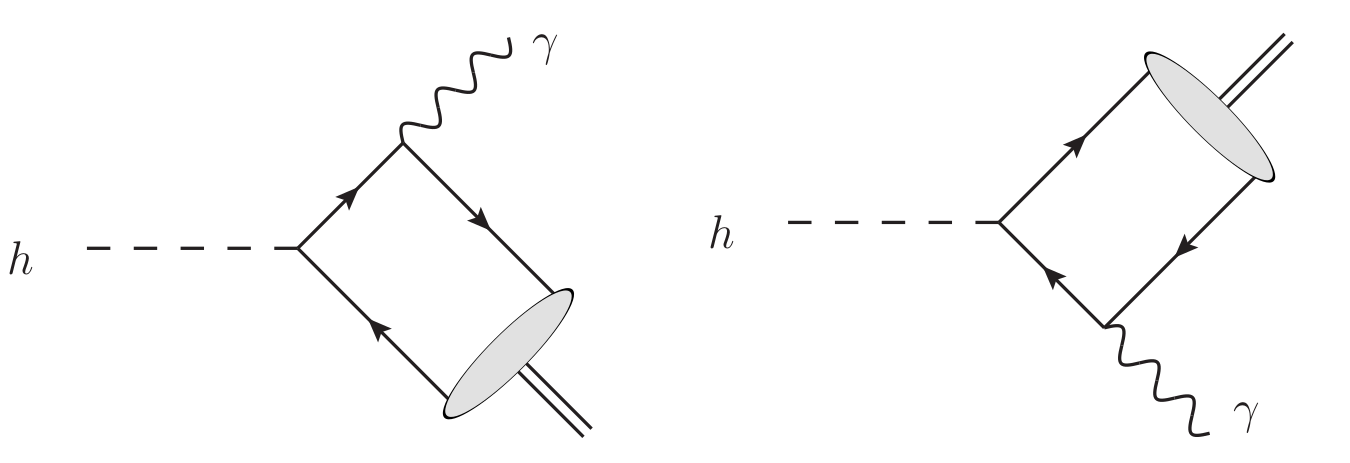
\includegraphics[height=1.2in]{figures/misc/Higgs_phirhoomega_direct.png}
			\caption{Direct contributions via Yukawa coupling to the light quarks.}
		\end{subfigure}
		\hfill
		\begin{subfigure}[t]{0.48\linewidth}
			\centering
			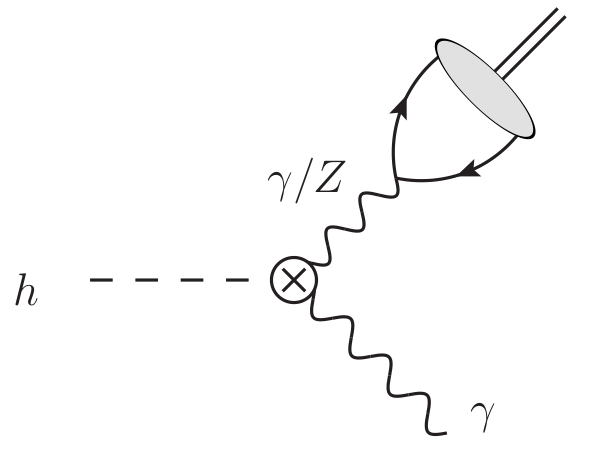
\includegraphics[height=1.2in]{figures/misc/Higgs_phirhoomega_indirect.png}
			\caption{Indirect contribution via a virtual photon or \(Z\) boson.}
		\end{subfigure}
		\caption{Leading order Feynman diagrams to the \(H\rightarrow M\gamma\) processes. Image taken from Fig. 2 of \cite{K_nig_2015}.}
	\end{figure}
\end{frame}

% Motivations (flavor-conserving, flavor-changing)
\begin{frame}{Motivations}
	\begin{columns}
		\begin{column}{0.4\textwidth}
			\textbf{Flavor-conserving probes}
			\begin{itemize}
				\item \(\PGf\): \(\PQs\) quark coupling (diagrams above)
				\item \(\PGrz\): \(\PQu\) and \(\PQd\) quark coupling
			\end{itemize}
			\vspace{1em}
			\textbf{Flavor-changing probe}
			\begin{itemize}
				\item \(\PKstarz\): flavor-changing \(\PQs\) and \(\PQd\) quarks via weak interaction (diagrams below)
			\end{itemize}
		\end{column}
		\begin{column}{0.5\textwidth}
			\begin{figure}
				\centering
				\kmfig{fig1}{height=0.75\textheight}
				\caption{Feynman diagrams showing the different Higgs boson decay mechanisms into a photon and a light meson (top: \(\PGf\) meson; bottom: \(\PKstarz\) meson).}
			\end{figure}
		\end{column}
	\end{columns}
\end{frame}

%%%%%% 2. Section: Introduction %%%%%%
\begin{frame}
	\vfill
	\centering
	\begin{beamercolorbox}[sep=8pt,center,shadow=false,rounded=true]{title}
		\usebeamerfont{title}\Huge Introduction \par%
	\end{beamercolorbox}
	\vfill
\end{frame}

% Strategy (final states)
\begin{frame}{Strategy}
	\begin{itemize}
		\item \khl{Final states}
		\begin{enumerate}
			\item High energy \textbf{photon}
			\item High energy \textbf{ditrack} from meson
			\item \ktodo{Look for photon-meson inv. mass}
		\end{enumerate}
	\end{itemize}
\end{frame}

% Strategy (production)
\begin{frame}{Strategy}
	\begin{itemize}
		\item \khl{Higgs Production Categories}
		\vspace{1em}
		\begin{columns}
			\centering
			\begin{column}{0.31\textwidth}
				\centering
				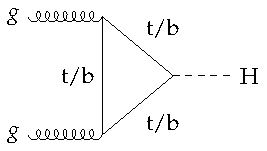
\includegraphics[height=0.25\textheight]{feynman-diagrams/ggH.pdf}\\
				\textbf{ggH}
				\begin{itemize}
					\item No \(e/\mu\)
					\item Veto events with \(|\Delta\eta_{JJ}| > 3\)
				\end{itemize}
			\end{column}
			\begin{column}{0.31\textwidth}
				\centering
				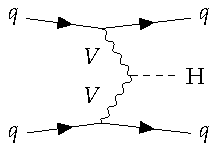
\includegraphics[height=0.25\textheight]{feynman-diagrams/VBF.pdf}\\
				\textbf{VBF high \(p_T^\gamma\)}
				\begin{itemize}
					\item Barrel photon \(p_T^\gamma > 75\) GeV
					\item No \(e/\mu\)
					\item \(|\Delta\eta_{JJ}| > 3\), \(M_{JJ} > 400\) GeV
				\end{itemize}
				\vspace{1em}
				\textbf{VBF low \(p_T^\gamma\)}
				\begin{itemize}
					\item \(40 < p_T^\gamma < 75\) GeV
					\item No \(e/\mu\)
					\item \(|\Delta\eta_{JJ}| > 3\), \(M_{JJ} > 300\) GeV
				\end{itemize}
			\end{column}
			\begin{column}{0.31\textwidth}
				\centering
				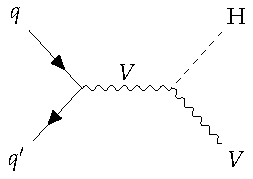
\includegraphics[height=0.25\textheight]{feynman-diagrams/VH.pdf}\\
				\textbf{VH (\(\mathbf{Z_{ll}H},\mathbf{W_{l\nu}H}\))}
				\begin{itemize}
					\item At least one \(l, \nu\)
					\item Also included is \(\mathbf{t\bar{t}H}\), accounting for \(\sim30\%\).
				\end{itemize}
			\end{column}
		\end{columns}
	\end{itemize}
\end{frame}

% Triggers
\begin{frame}{Triggers}
	\begin{itemize}
		\item {\color{red}What to discuss?}
		\item \ktodo{Trigger efficiency --- how to measure (slide with plots)}
		\begin{itemize}
			\item \(Z\rightarrow \mu^+\mu^-\) events data/MC
			\item Measure photon leg \& tau leg
			\item Figs. 30 \& 38
		\end{itemize}
	\end{itemize}
	\begin{table}
		\centering
		\small
		\begin{tabular}{|l|c|c|c|c|}
			\hline
			& \textbf{ggH} & \textbf{High-\(\mathbf{p^\gamma_T}\) VBF} & \textbf{Low-\(\mathbf{p^\gamma_T}\) VBF} & \textbf{VH} \\
			\hline
			& & & & single/di-muon\\
			Triggers & tau-like & VBF-like & tau-like & single/di-electron\\
			& & & & muon+gamma\\
			\hline
			& & 28.2 (2016) & & \\
			Luminosity (\(\mathrm{fb^{-1}}\)) & 39.50 (2018) & 7.7 (2017) & 39.50 (2018) & 138 (2016--2018) \\
			& & 60 (2018) & & \\
			\hline	
		\end{tabular}
	\end{table}
\end{frame}

% Simulated Samples
\begin{frame}{Simulated Samples}
	\begin{align*}
		\phi(1020)&\rightarrow K^+K^-\;\;(\mathrm{BR} \sim 49\%)\\
		\rho(770)&\rightarrow \pi^+\pi^-\;\;(\mathrm{BR} \sim 100\%)\\
		K^*_0(892)&\rightarrow K^\pm\pi^\mp\;\;(\mathrm{BR} \sim 100\%)
	\end{align*}
	\ktodo{Polarization reweighting (new slide if plot)}
\end{frame}

% Event Selection (photon selection)
\begin{frame}{Event Selection}
	\begin{itemize}
		\item \khl{Photon selection}
		\vspace{1em}
		\begin{table}[!ht]
			\centering
			\small
			\begin{tabular}{|l|c|c|c|c|}
				\hline
				& \multicolumn{1}{C{8em}}{\textbf{ggH}} & \multicolumn{1}{C{8em}}{\textbf{High-\(\mathbf{p^\gamma_T}\) VBF}} & \multicolumn{1}{C{8em}}{\textbf{Low-\(\mathbf{p^\gamma_T}\) VBF}} &  \multicolumn{1}{C{8em}|}{\textbf{VH}} \\
				\hline
				\(p^\gamma_T\) [GeV] & \multicolumn{1}{C{8em}}{\(> 38\)} & \multicolumn{1}{C{8em}}{\(> 75\)} & \multicolumn{1}{C{8em}}{\(38 < p^\gamma_T < 75\)} & \multicolumn{1}{C{8em}|}{\(> 40\)}\\
				\(|\eta^\gamma|\) & \multicolumn{1}{C{8em}}{\(< 2.1\)} & \multicolumn{1}{C{8em}}{\(< 1.4\)} & \multicolumn{1}{C{8em}}{\(< 2.1\)} & \multicolumn{1}{C{8em}|}{\(< 2.5\)}\\
				\(\gamma\)-ID signal eff. & \multicolumn{1}{C{8em}}{\(80\%\)} & \multicolumn{1}{C{8em}}{\(90\%\)} & \multicolumn{1}{C{8em}}{\(80\%\)} & \multicolumn{1}{C{8em}|}{\(90\%\)}\\
				\hline
			\end{tabular}
			\caption{Photon selection criteria across different production categories.}
		\end{table}
		\begin{itemize}
			\item \(\gamma\)-ID signal eff. = MVA-based selection ID \cite{photon_mvaid}
			\item \(p^\gamma_T\) cut based on trigger
			\item {\color{red}Where is the information about di-photon veto for ggH?} \ktodo{ggH \& VH}.
			\item ggH/VBF: conversion veto, VH: pixel veto.
			\item Highest-\(p^\gamma_T\) photon chosen as candidate.
		\end{itemize}
	\end{itemize}
\end{frame}

% Event Selection (di-track)
\begin{frame}{Event Selection}
	\begin{columns}
		\begin{column}{0.5\textwidth}
			\begin{itemize}
				\item \khl{Ditrack reconstruction}\\
				\begin{itemize}
					\item Track selection
					\begin{enumerate}
						\item Originate from PV
						\item Pass ``high purity" criteria
					\end{enumerate}
					\item Meson definition (\(M=\phi, \rho^0, K^*_0\))
					\begin{enumerate}
						\item Pair of oppositely charged tracks
						\item \(p_T > 5\) GeV, \(|\eta| < 2.5\)
						\item At least one track \(p_T > 20\) GeV
					\end{enumerate}
					\item Invariant mass
					\begin{enumerate}
						\item \(\rho^0: 0.62 < m_{\pi\pi} < 0.92\) GeV\\
						\(\phi: 1.008 < m_{KK} < 1.032\) GeV\\
						\(K^*_0: 0.84 < m_{K\pi} < 0.94\) GeV
						\item \(m_{K\pi}\) closest to \(m_{K^*_0}\) selected
						\item Reject events where \(m_{KK}\) consistent with \(m_{\phi}\) and have higher \(p_T\), vice versa.
					\end{enumerate}
				\end{itemize}
			\end{itemize}
		\end{column}
		\begin{column}{0.35\textwidth}
		\end{column}
	\end{columns}
	\vspace{1em}
	\begin{center}
		\khl{Applies to all production categories.}
	\end{center}
\end{frame}

\begin{frame}{Event Selection}
	\ktodo{mass sidebands}
\end{frame}

% Event selection (di-track system)
\begin{frame}{Event Selection}
	\begin{itemize}
		\item \khl{Di-track system}\\
		Define the relative \textbf{charged isolation} of the leading meson candidate,
		\begin{align*}
			I^{\mathrm{trk}}(M) = \frac{p_T^{M}}{p_T^{M} + {\color{Plum}\sum_{trk}|p_T^{trk}|}}\,,
		\end{align*}
		and the \textbf{neutral isolation} as
		\begin{align*}
			I^{\mathrm{neu}}(M) = \frac{p_T^{M}}{p_T^{M} + {\color{Plum}\sum_{neu}|p_T^{neu}|}}\,.
		\end{align*}
		\({\color{Plum}\sum_{trk/neu}|p_T^{trk/neu}|}\) {: \color{Plum}sum of charged/neutral track \(p_T\) within \(\Delta R = 0.3\)} of meson candidate.
		\vspace{1em}
		\begin{table}[!ht]
			\centering
			\small
			\begin{tabular}{|l|c|c|c|c|}
				\hline
				& \multicolumn{1}{C{8em}}{\textbf{ggH}} & \multicolumn{1}{C{8em}}{\textbf{High-\(\mathbf{p^\gamma_T}\) VBF}} & \multicolumn{1}{C{8em}}{\textbf{Low-\(\mathbf{p^\gamma_T}\) VBF}} &  \multicolumn{1}{C{8em}|}{\textbf{VH}} \\
				\hline
				\(p^M_T\) [GeV] & \multicolumn{1}{C{8em}}{\(> 38\)} & \multicolumn{1}{C{8em}}{\(> 40\)} & \multicolumn{1}{C{8em}}{\(> 40\)} & \multicolumn{1}{C{8em}|}{\(> 40\)}\\
				\(I^{trk}_M\) & \multicolumn{1}{C{8em}}{\(> 0.9\)} & \multicolumn{1}{C{8em}}{\(> 0.9\)} & \multicolumn{1}{C{8em}}{\(> 0.9\)} & \multicolumn{1}{C{8em}|}{\(> 0.8\)}\\
				\(I^{neu}_M\) & \multicolumn{1}{C{8em}}{\(> 0.8\)} & \multicolumn{1}{C{8em}}{-} & \multicolumn{1}{C{8em}}{-} & \multicolumn{1}{C{8em}|}{-}\\
				\hline
			\end{tabular}
			\caption{Di-track system criteria across different production categories.}
		\end{table}
		\begin{itemize}
			\item Highest-\(p_T\) meson chosen as candidate.
		\end{itemize}
	\end{itemize}
\end{frame}

% Event Selection (event tagging)
\begin{frame}{Event Selection}
	\begin{itemize}
		\item \khl{Event tagging}
		\vspace{1em}
		\begin{table}[!ht]
			\centering
			\small
			\begin{tabular}{|l|c|c|c|c|}
				\hline
				& \multicolumn{1}{C{8em}}{\textbf{ggH}} & \multicolumn{1}{C{8em}}{\textbf{High-\(\mathbf{p^\gamma_T}\) VBF}} & \multicolumn{1}{C{8em}}{\textbf{Low-\(\mathbf{p^\gamma_T}\) VBF}} &  \multicolumn{1}{C{8em}|}{\textbf{VH}} \\
				\hline
				Event tagging & \multicolumn{1}{C{8em}}{Meson candidate within a jet with \(p_T^\mathrm{j} > 40\) GeV, tracks with \(\Delta R < 0.07\)} & \multicolumn{1}{C{8em}}{2 jets with \(p_T^{j} > 40\) GeV, \(m_{jj} > 400\) GeV, \(\eta_{jj} > 3\)} & \multicolumn{1}{C{8em}}{2 jets with \(p_T^{j} > 30, 20\) GeV, \(m_{jj} > 300\) GeV, \(\eta_{jj} > 3\)} & \multicolumn{1}{C{8em}|}{1 selected and isolated \(e/\mu\) or 2 selected \(e/\mu\) compatible with \(m_Z\)}\\
				\hline
			\end{tabular}
			\caption{Event tagging selection criteria across different production categories.}
		\end{table}
		\begin{itemize}
			\item 
		\end{itemize}
	\end{itemize}
\end{frame}

% Event Selection (non-MVA summary)
\begin{frame}{Event Selection}
	
	\khl{Summary of Event Selection}
	\vspace{0.2em}
	\ktodo{Take the version of the paper}
	\begin{table}[!ht]
		\centering
		\footnotesize
		\begin{tabular}{|l|c|c|c|c|}
			\hhline{|=====|}
			& \multicolumn{4}{c|}{\textbf{Common selections}}\\
			\hhline{|=====|}
			& \multicolumn{4}{C{36em}|}{``high-purity" tracks, opposite sign} \\
			M selection & \multicolumn{4}{C{36em}|}{\(|\eta^{\mathrm{trk}}| < 2.5\),  \(p_T^{\mathrm{trk1}} > 20\) GeV,   \(p_T^{\mathrm{trk1}} > 5\) GeV,  \(|\eta^M| < 2.1\)} \\
			& \multicolumn{4}{C{36em}|}{\(0.62 < m_{\pi\pi} < 0.92\) GeV,  \(1.008 < m_{KK} < 1.032\) GeV,  \(0.84 < m_{K\pi} < 0.94\) GeV} \\
			\hhline{|=====|}
			% categories
			& \multicolumn{1}{C{8em}}{\textbf{ggH}} & \multicolumn{1}{C{8em}}{\textbf{High-\(\mathbf{p^\gamma_T}\) VBF}} & \multicolumn{1}{C{8em}}{\textbf{Low-\(\mathbf{p^\gamma_T}\) VBF}} &  \multicolumn{1}{C{8em}|}{\textbf{VH}} \\
			\hline
			% Photon
			\(p^\gamma_T\) [GeV] & \multicolumn{1}{C{8em}}{\(> 38\)} & \multicolumn{1}{C{8em}}{\(> 75\)} & \multicolumn{1}{C{8em}}{\(40 < p^\gamma_T < 75\)} & \multicolumn{1}{C{8em}|}{\(> 40\)}\\
			\(|\eta^\gamma|\) & \multicolumn{1}{C{8em}}{\(< 2.1\)} & \multicolumn{1}{C{8em}}{\(< 1.4\)} & \multicolumn{1}{C{8em}}{\(< 2.1\)} & \multicolumn{1}{C{8em}|}{\(< 2.5\)}\\
			\(\gamma\)-ID signal eff. & \multicolumn{1}{C{8em}}{\(80\%\)} & \multicolumn{1}{C{8em}}{\(90\%\)} & \multicolumn{1}{C{8em}}{\(80\%\) (endcap), \(90\%\) (barrel)} & \multicolumn{1}{C{8em}|}{\(90\%\)}\\
			\hline
			% Di-track
			\(p^M_T\) [GeV] & \multicolumn{1}{C{8em}}{\(> 38\)} & \multicolumn{1}{C{8em}}{\(> 40\)} & \multicolumn{1}{C{8em}}{\(> 40\)} & \multicolumn{1}{C{8em}|}{\(> 40\)}\\
			\(I^{trk}_M\) & \multicolumn{1}{C{8em}}{\(> 0.9\)} & \multicolumn{1}{C{8em}}{\(> 0.9\)} & \multicolumn{1}{C{8em}}{\(> 0.9\)} & \multicolumn{1}{C{8em}|}{\(> 0.8\)}\\
			\(I^{neu}_M\) & \multicolumn{1}{C{8em}}{\(> 0.8\)} & \multicolumn{1}{C{8em}}{-} & \multicolumn{1}{C{8em}}{-} & \multicolumn{1}{C{8em}|}{-}\\
			\hline
			% Event tagging
			Event tagging & \multicolumn{1}{C{8em}}{Meson candidate within a jet with \(p_T^\mathrm{j} > 40\) GeV, tracks with \(\Delta R < 0.07\)} & \multicolumn{1}{C{8em}}{2 jets with \(p_T^{j} > 40\) GeV, \(m_{jj} > 400\) GeV, \(\eta_{jj} > 3\)} & \multicolumn{1}{C{8em}}{2 jets with \(p_T^{j} > 30, 20\) GeV, \(m_{jj} > 300\) GeV, \(\eta_{jj} > 3\)} & \multicolumn{1}{C{8em}|}{1 selected and isolated \(e/\mu\) or 2 selected \(e/\mu\) compatible with \(m_Z\)}\\
			\hline
		\end{tabular}
		\caption{\ktodo{Taken from paper} Summary of event selection before MVA.}
	\end{table}
\end{frame}

% MC/data background
\begin{frame}{MC/Data Background Comparison}
	content...
\end{frame}

% MVA (overview)
\begin{frame}{Event Selection (MVA)}
	\begin{itemize}
		\item \khl{Multivariate Analysis (MVA)}
		\vspace{1em}
		\begin{itemize}
			\item BDT classifiers based on ROOT TMVA \cite{hoecker2009tmva} for \textbf{ggH}, \textbf{low-\(\mathbf{p^\gamma_T}\) VBF}, and \textbf{high-\(\mathbf{p^\gamma_T}\) VBF}.
			\item Training and validation samples defined by \textbf{meson mass SR \& sidebands}.
			\item Signal \& Background events weighted by \(1/(\sigma_M/M)\), where
			\begin{align*}
				\frac{\sigma_M}{M} = \sqrt{\left(\frac{\sigma_m}{m}\right)^2_{\mathrm{meson}} + \left(\frac{\sigma _E}{E}\right)^2_{\mathrm{\gamma}}}
			\end{align*}
		\end{itemize}
	\end{itemize}
\end{frame}

% MVA (overview-variables)
\begin{frame}{Event Selection (MVA)}
	\begin{itemize}
		\item \khl{Multivariate Analysis (MVA)}
		\vspace{1em}
		\begin{itemize}
			\item Input variables used for ggH and VBF categories.
			\begin{table}
				\centering
				\begin{tabular}{l | c | c | c }
					& \multicolumn{1}{C{8em}|}{\textbf{ggH}} & \multicolumn{1}{C{8em}|}{\textbf{High-\(\mathbf{p^\gamma_T}\) VBF}} & \multicolumn{1}{C{8em}}{\textbf{Low-\(\mathbf{p^\gamma_T}\) VBF}} \\
					\hline
					& & \(p^{M\gamma}_T\) & \(p^{M\gamma}_T\) \\
					Kinematics & \(p^{\gamma}_T\) & \(p^{\gamma}_T\) & \(p^{\gamma}_T\) \\
					& \(p^{M}_T\) & \(p^{M}_T/m_{M\gamma}\) & \(p^{M}_T/m_{M\gamma}\) \\
					 & \(\eta_M\) & & \\
					\hline
					Meson Isolation & \(I^{\mathrm{trk}}(M)\) & \(I^{\mathrm{trk}}(M)\) & \(I^{\mathrm{trk}}(M)\) \\
					\hline
					& & \(M_{JJ}\) & \(M_{JJ}\) \\
					Jet-related & & \(\Delta\phi_{JJ}\) & \(\Delta\phi_{JJ}\) \\
					& & \ktodo{zepVar} & \ktodo{zepVar} \\
				\end{tabular}
			\end{table}
		\end{itemize}
	\end{itemize}
\end{frame}

% MVA (ggH)
\begin{frame}{Event Selection (MVA)}
	\begin{itemize}
		\item \khl{Multivariate Analysis (MVA): ggH category}
		\vspace{1em}
		\begin{itemize}
			\item Input variables
			\item SR \& CR
			\item Results.
			\item MVAdisc
			\item cat0 \& cat1
		\end{itemize}
	\end{itemize}
\end{frame}

% MVA (VBF high)
\begin{frame}{Event Selection (MVA)}
	\begin{itemize}
		\item \khl{Multivariate Analysis (MVA): High-\(p^\gamma_T\) VBF category}
		\vspace{1em}
		\begin{itemize}
			\item Input variables
			\item SR \& CR
			\item Results.
			\item MVAdisc
		\end{itemize}
	\end{itemize}
\end{frame}

% MVA (VBF low)
\begin{frame}{Event Selection (MVA)}
	\begin{itemize}
		\item \khl{Multivariate Analysis (MVA): Low-\(p^\gamma_T\) VBF category}
		\vspace{1em}
		\begin{itemize}
			\item Input variables
			\item SR \& CR
			\item Results.
			\item MVAdisc
		\end{itemize}
	\end{itemize}
\end{frame}

% 
\begin{frame}
	content...
\end{frame}

% 
\begin{frame}
	content...
\end{frame}

% Systematic uncertainties
\begin{frame}{Systematic Uncertainties}
	\ktodo{Note: only for signal}
	\begin{enumerate}
		\item \textbf{Integrated Luminosity}
		\item \textbf{Total inelastic cross section} correcting PU profile in simulation to data.
		\item \textbf{Trigger efficiencies}.
		\item \textbf{Photon ID efficiencies}. Derived from \(Z\rightarrow e^+e^-\).
		\item \textbf{Tracking efficiency}.
		\item \textbf{Muon/Electron ID}.
		\item \textbf{Meson Charged/Neutral Isolation Efficiencies}.
		\item \textbf{JEC \& JES}\\
		\vspace{1em}
		Theoretical:\\
		\item \textbf{QCD renormalization and factorization}.
		\item \textbf{PDF \& \(\mathbf{\alpha_S}\)}.
		\item \textbf{Parton shower modeling} from renormalization of QCD-induced ISR and FSR in \texttt{PYTHIA}.
	\end{enumerate}
\end{frame}

% Signal modeling
\begin{frame}{Signal modeling}
	\begin{itemize}
		\item \khl{\(\mathbf{m_{M\gamma}}\)}. Distribution of the \khl{reconstructed Higgs boson mass}.
		\item Analytic function: \textbf{two-tailed Crystal Ball(TTCB)}.
		\begin{align*}
			\label{eq:ttcb}
			\mathrm{TTCB}(t) = \left\{
			\begin{array}{l l}
				e^{-t^2/2}, & \mathrm{for}~~-\alpha_L<t<\alpha_R\\
				(\frac{n_L}{|\alpha_L|})^{n_{L}}e^{-\alpha_L^2/2}(\frac{n_L}{|\alpha_L|}-|\alpha_L|-t)^{-n_{L}}, & \mathrm{for}~~t\leq-\alpha_L\\
				(\frac{n_R}{|\alpha_R|})^{n_{R}}e^{-\alpha_R^2/2}(\frac{n_R}{|\alpha_R|}-|\alpha_R|+t)^{-n_{R}}, & \mathrm{for}~~t\geq\alpha_L\\
			\end{array} \right.
		\end{align*}
		\item Fitted via unbinned likelihood to simulated signal events.
	\end{itemize}
\end{frame}

% Background modeling
\begin{frame}{Background modeling}
	\begin{itemize}
		\item Analytic functions: \textbf{Chebychev} polynomials (main), \textbf{Bernstein} polynomials and \textbf{exponential} series (determination of shape uncertainties).
		\item Fitting region defined as \(m_{M\gamma}\) sidebands.\\
		\begin{itemize}
			\item ggH category: \(110 < m_{M\gamma} < 120\) GeV \& \(130 < m_{M\gamma} < 160\) GeV. 
			\item VBF categories (high \& low \(p^\gamma_T\)): \(100 < m_{M\gamma} < 120\) GeV \& \(130 < m_{M\gamma} < 170\) GeV.
			\item VH category: \(100 < m_{M\gamma} < 120\) GeV \& \(130 < m_{M\gamma} < 150\) GeV.
		\end{itemize}
		\item Degree of polynomial determined with \textbf{F-test}.
		\item \textbf{Bias test}.
	\end{itemize}
\end{frame}

% Signal & Background fits
\begin{frame}{Signal \& Background Post-fit Distributions}
	content...
\end{frame}

% Unblinded limits (methodology)
\begin{frame}{Results}
	\begin{itemize}
		\item \khl{Upper limits} on $\mathcal{B}(H\rightarrow\rho^0\gamma)$, $\mathcal{B}(H\rightarrow\phi\gamma)$, and $\mathcal{B}(H\rightarrow K^*_0\gamma)$ set at 95\% CL.
		\item CLs profile-likelihood ratio used as test-statistics, with the asymptotic approximation.
		\item Systematic uncertainties treated as nuisance parameters. 
	\end{itemize}
\end{frame}

% Unblinded limits (bands)
\begin{frame}{Results}
	\begin{figure}
		\begin{subfigure}{.36\textwidth}
			\centering
			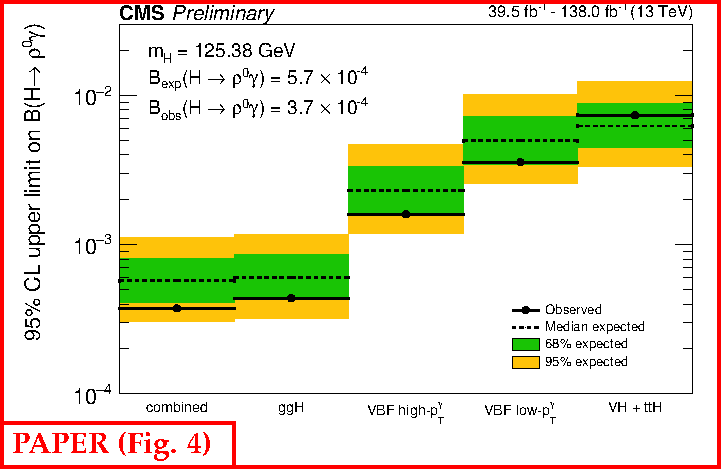
\includegraphics[width=\textwidth]{figures/23-005-v07-marked-figs/fig4-top-right.pdf}
		\end{subfigure}%
		\begin{subfigure}{.36\textwidth}
			\centering
			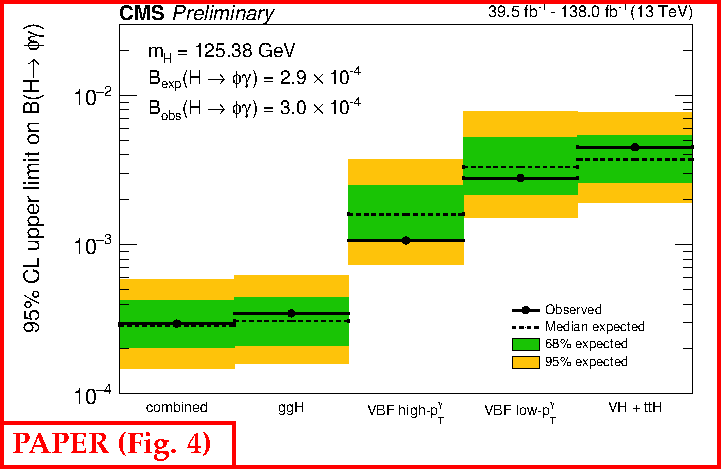
\includegraphics[width=\textwidth]{figures/23-005-v07-marked-figs/fig4-top-left.pdf}
		\end{subfigure}\\
		\begin{subfigure}{.36\textwidth}
			\centering
			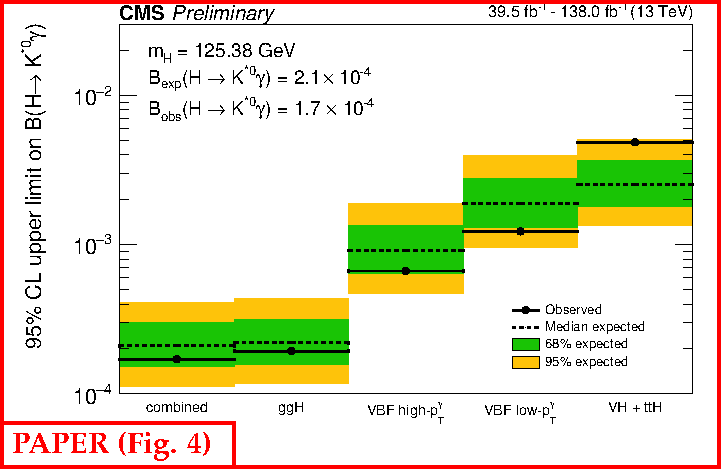
\includegraphics[width=\textwidth]{figures/23-005-v07-marked-figs/fig4-bottom.pdf}
		\end{subfigure}
		\vspace{0.1em}
		\caption{Expected and observed upper limits on $\mathcal{B}(H\rightarrow\rho^0\gamma)$ (top left), $\mathcal{B}(H\rightarrow\phi\gamma)$ (top right), and $\mathcal{B}(H\rightarrow K^*_0\gamma)$ (bottom) split by analysis categories and combined. Green and yellow bands correspond to 1 and 2$\sigma$ confidence intervals in the expected upper limits.}
	\end{figure}
\end{frame}

% Unblinded limits (table)
\begin{frame}{Results}
	\begin{table}
		\centering
		\begin{tabular}{lrrrrrr}
			\hline
			& \multicolumn{2}{c}{U.L. $\mathcal{B}(H\rightarrow \rho^0\gamma)$}  & \multicolumn{2}{c}{U.L. $\mathcal{B}(H\rightarrow \phi\gamma)$} &  \multicolumn{2}{c}{U.L. $\mathcal{B}(H\rightarrow K^*_0\gamma)$}\\ [2ex]
			category & Exp.$(10^{-4})$ & Obs.$(10^{-4})$ & Exp.$(10^{-4})$ & Obs.$(10^{-4})$ & Exp.$(10^{-4})$ & Obs.$(10^{-4})$\\
			\hline
			VH & $62.3^{+25.6}_{-17.9}$ & 73.7 & $37.3^{+16.9}_{-11.3}$ & 45.0 & $25.3^{+11.4}_{-7.3}$ & 48.5 \\[2ex]
			low-$p_T^\gamma$ VBF & $49.6^{+22.5}_{-15.0}$ & 35.6 & $33.1^{+18.7}_{-11.5}$ & 27.9 & $18.8^{+8.90}_{-5.7}$  & 12.3\\[2ex]
			high-$p_T^\gamma$ VBF & $22.9^{+10.5}_{-6.9}$ & 16.0 & $16.0^{+9.0}_{-5.5}$ & 10.7 & $9.13^{+4.25}_{-2.75}$ & 6.66 \\[2ex]
			ggH &$6.01^{+2.53}_{-1.72}$ & 4.37 & $3.08^{+1.33}_{-0.98}$ & 3.46 & $2.20^{+0.94}_{-0.62}$ & 1.93\\ [2ex]
			\cellcolor{orange!50}\textbf{combined} & \cellcolor{orange!50}$5.71^{+2.37}_{-1.63}$ & \cellcolor{orange!50}\textbf{3.74} & \cellcolor{orange!50} $2.88^{+1.33}_{-0.83}$ & \cellcolor{orange!50} \textbf{2.97} & \cellcolor{orange!50}$2.10^{+0.90}_{-0.58}$ & \cellcolor{orange!50}\textbf{1.71} \\[2ex]
			\hline
		\end{tabular}
		\caption{Exclusion limits at 95\% CL on the branching fractions of the H boson decays. Observed and median expected limits with the upper and lower bounds in the expected 68\% CL intervals are reported.}
	\end{table}
\end{frame}

\begin{frame}{Results}
	\begin{table}[!ht]
		\centering
		\begin{tabular}[t]{|l|c|c|l|l|}
			\hline
			\multicolumn{1}{|c|}{\cellcolor{lightgray}\small Channel} & \cellcolor{lightgray}\small Coupling & \cellcolor{lightgray}\small SM \(\mathcal{BR}(\htomg)\) & \multicolumn{1}{c|}{\cellcolor{lightgray}\small Limits on \(\mathcal{BR}\)} & \multicolumn{1}{c|}{\cellcolor{lightgray}\small Notes} \\
			\hline
			
			% phi
			\multirow{2}{*}{\(\Hgphi\)} & \multirow{2}{*}{\(s\)} & \multirow{2}{*}{\((1.68\pm0.08) \times 10^{-5}\)\cite{K_nig_2015}} & Exp. \(4.2^{+1.8}_{-1.2}\times10^{-4}\) & ATLAS Run 2, \(35.6\;\textrm{fb}^{-1}\) \\ & & & Obs. \(5.0\times10^{-4}\) \cite{ATLAS_rhophigamma2023} & \(\phi\gamma\rightarrow K^+K^-\gamma\)\\
			\hline
			
			% rho
			\multirow{2}{*}{\(\Hgphi\)} & \multirow{2}{*}{\(u, d\)} & \multirow{2}{*}{\((2.31\pm0.11) \times 10^{-6}\)\cite{K_nig_2015}} & Exp. \(10.0^{+4.9}_{-2.8}\times10^{-4}\) & ATLAS Run 2, \(35.6\;\textrm{fb}^{-1}\) \\ & & & Obs. \(10.4\times10^{-4}\) \cite{ATLAS_rhophigamma2023} & \(\rho\gamma\rightarrow \pi^+\pi^-\gamma\) \\
			\hline
			
			% K0star
			\multirow{2}{*}{\(\Hgkstar\)} & & \tiny (Only available for \(\PH\to \PQd\PAQs + \PAQd\PQs\)) & Exp. \(3.7^{+1.5}_{-1.0}\times10^{-4}\) & ATLAS Run 2, \(134\;\textrm{fb}^{-1}\) \\ & \multirow{-2}{*}{\(d\&s\) (flavor-changing)} & \(1.19\times10^{-11}\) \cite{Aranda_2020} & Obs. \(2.2\times10^{-4}\) \cite{ATLAS_omegaK0stargamma} & \(K^*_0\gamma\rightarrow K^\pm\pi^\mp\gamma\) \\
			\hline
		\end{tabular}
		\caption{\(\htomg\) channels considered in this analysis with their respective couplings and predicted branching ratios.}
		\label{tab:Higgs_rare_decays_results}
	\end{table}
\end{frame}

%%%%%%%%%%%%%% BACKUP %%%%%%%%%%%%%%%%%%
% Important: comparison with ATLAS (backup)

\begin{frame}{Bibliography}
	\scriptsize
	\bibliographystyle{JHEP}
	\bibliography{refs.bib}
\end{frame}
\end{document}
